%%%%%%%%%%%%%%%%%%%%%%%%%%%%%%%%%%%%%%%%%%%%%%%%%%%%%%%%%%%%%%%%%%%%%%%%%%%%%%%%%%
\begin{frame}[fragile]\frametitle{}
\begin{center}
{\Large Overview of Large Language Models}
\end{center}
\end{frame}

%%%%%%%%%%%%%%%%%%%%%%%%%%%%%%%%%%%%%%%%%%%%%%%%%%%%%%%%%%%
\begin{frame}[fragile]\frametitle{What is a Language Models?}

\begin{itemize}
\item While typing SMS, have you seen it suggests next word?
\item While typing email, have you seen next few words are suggested?
\item How does it suggest? (suggestions are not random, right?)
\item In the past, for ``Lets go for a \ldots', if you have typed 'coffee' 15 times, 'movie' say 4 times, then it learns that. Machine/Statistical Learning.
\item Next time, when you type ``Lets go for a '', what will be suggested? why?
\item This is called Language Model. Predicting the next word. When done continuously, one after other, it spits sentence, called Generative Model.
\end{itemize}	

\begin{center}
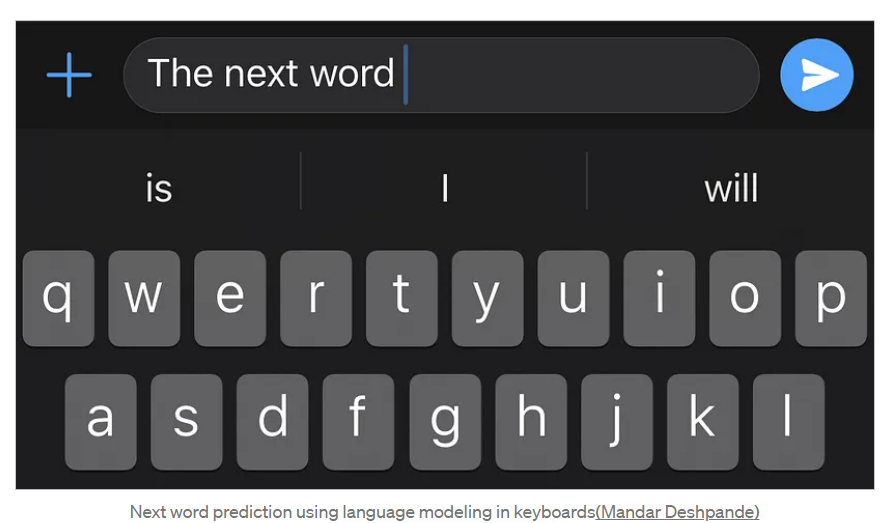
\includegraphics[width=0.6\linewidth,keepaspectratio]{chatgpt34}
\end{center}		

\end{frame}

%%%%%%%%%%%%%%%%%%%%%%%%%%%%%%%%%%%%%%%%%%%%%%%%%%%%%%%%%%%
\begin{frame}[fragile]\frametitle{Overview}


\begin{itemize}
\item Large Language Models (LLMs) are deep neural networks (e.g., GPT-3, BERT) based on the Transformer architecture.
\item LLMs are foundation models trained on large amounts of unsupervised and unstructured data.
\item The Transformer architecture consists of an encoder and decoder, both mostly identical with a few differences.
\item LLMs compute a probability distribution over a vocabulary (list of tokens) given an input prompt.
\item LLMs have limitations like hallucination and issues in chain of thought reasoning, but recent improvements have been made.
\item LLMs are trained for statistical language modeling, which involves predicting the next token based on context.
\end{itemize}

				
{\tiny (Ref: Overview of Large Language Models - Aman AI)}

\end{frame}


%%%%%%%%%%%%%%%%%%%%%%%%%%%%%%%%%%%%%%%%%%%%%%%%%%%%%%%%%%%
\begin{frame}[fragile]\frametitle{Evolution of Language Models}

Language Models can be statistical (frequency based) or Machine/Deep Learning (supervised) based. Simple to complex.

\begin{center}
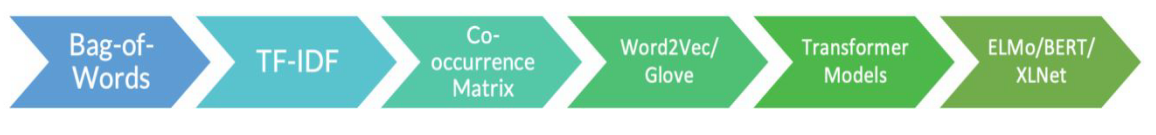
\includegraphics[width=\linewidth,keepaspectratio]{chatgpt30}
\end{center}				
{\tiny (Ref: Analytics Vidhya https://editor.analyticsvidhya.com/uploads/59483evolution\_of\_NLP.png)}

\end{frame}

%%%%%%%%%%%%%%%%%%%%%%%%%%%%%%%%%%%%%%%%%%%%%%%%%%%%%%%%%%%
\begin{frame}[fragile]\frametitle{Large Language Models - Comparison}

\begin{center}
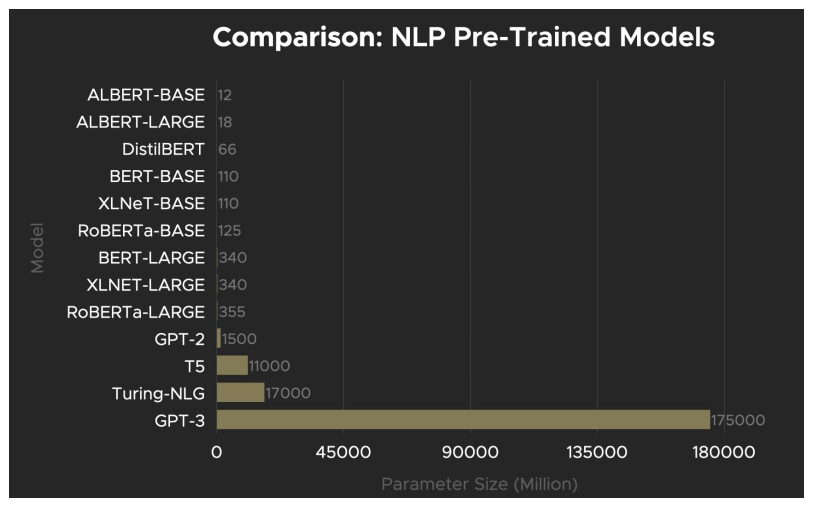
\includegraphics[width=\linewidth,keepaspectratio]{chatgpt31}
\end{center}				
{\tiny (Ref: Deus.ai https://www.deus.ai/post/gpt-3-what-is-all-the-excitement-about)}

\end{frame}

%%%%%%%%%%%%%%%%%%%%%%%%%%%%%%%%%%%%%%%%%%%%%%%%%%%%%%%%%%%
\begin{frame}[fragile]\frametitle{How Do LLMs Work?}


\begin{itemize}
\item LLMs predict the next token based on previous tokens in an autoregressive manner for generation.
\item The prompt is tokenized and converted into non-contextualized embeddings.
\item Layer-by-layer attention and feed-forward computations are performed.
\item Decoder models assign logits to words in the vocabulary or output contextualized embeddings for encoder models.
\item For decoder models, logits are converted into a probability distribution using Softmax.
\item The probability distribution determines the next word in the generated text.
\end{itemize}

				
{\tiny (Ref: Overview of Large Language Models - Aman AI)}

\end{frame}

%%%%%%%%%%%%%%%%%%%%%%%%%%%%%%%%%%%%%%%%%%%%%%%%%%%%%%%%%%%
\begin{frame}[fragile]\frametitle{LLM Training Steps}

At a top-level, here are steps involved in training LLMs:

\begin{itemize}
\item Corpus Preparation: Gather a large corpus of text data from various sources.
Tokenization: Split the text into individual words or subword units (tokens).
Embedding Generation: Generate embeddings using random initialization or pre-trained embeddings like Word2Vec, GloVe, or FastText.
Neural Network Training: Train a neural network model on the input tokens.
\begin{itemize}
\item For encoder models (e.g., BERT), predict the context of a given word through masked language modeling and next sentence prediction tasks.
\item For decoder models (e.g., GPT-N), predict the next token in the sequence based on prior context.
\end{itemize}
\end{itemize}

				
{\tiny (Ref: Overview of Large Language Models - Aman AI)}

\end{frame}

%%%%%%%%%%%%%%%%%%%%%%%%%%%%%%%%%%%%%%%%%%%%%%%%%%%%%%%%%%%
\begin{frame}[fragile]\frametitle{Computing Similarity Between Embeddings}


\begin{itemize}
\item Encoder models provide contextualized embeddings that enable arithmetic operations for various tasks.
\item Contextualized embeddings can be used for word similarity by comparing the embeddings of the respective words.
\item For sentence similarity, the output of the [CLS] token or the average of word embeddings can be used.
\item Sentence BERT variants of encoder models are preferred for optimal performance on sentence similarity tasks.
\item Word/sentence similarity measures the semantic equivalence between two words/sentences.
\item Two common measures of word/sentence similarity exist, which are not considered "distance metrics."
\end{itemize}

				
{\tiny (Ref: Overview of Large Language Models - Aman AI)}

\end{frame}


%%%%%%%%%%%%%%%%%%%%%%%%%%%%%%%%%%%%%%%%%%%%%%%%%%%%%%%%%%%
\begin{frame}[fragile]\frametitle{Reasoning}


\begin{itemize}
\item Reasoning in LLMs refers to the ability to make inferences using evidence and logic.
\item There are different types of reasoning, including commonsense reasoning and mathematical reasoning.
\item Various methods, such as prompting, can be used to elicit reasoning from LLMs.
\item Determining the extent of reasoning used by LLMs for final predictions is challenging, as separating reasoning from factual information is not straightforward.
\end{itemize}

				
{\tiny (Ref: Overview of Large Language Models - Aman AI)}

\end{frame}


%%%%%%%%%%%%%%%%%%%%%%%%%%%%%%%%%%%%%%%%%%%%%%%%%%%%%%%%%%%
\begin{frame}[fragile]\frametitle{GPTs Training}

GPT: Generative Pre-trained Transformers

\begin{itemize}
% \item GPT-1 is trained in a self-supervised manner (learn to predict the next word in text data) and fine-tuned in a supervised learning manner. 
% \item GPT-2 is trained in a fully self supervised way, focusing on zero-shot transfer
% \item  GPT-3 is pre-trained in a self supervised manner exploring a bit more the few-shots fine-tuning.
\item GPT-1 is pre-trained on the BooksCorpus dataset, containing ~7000 books amounting to ~5GB of data
\item GPT-2 is pre-trained using the WebText dataset which is a more diverse set of internet data containing ~8M documents for about ~40 GB of data
\item GPT-3 uses an expanded version of the WebText dataset, two internet-based books corpora that are not disclosed and the English-language Wikipedia which constituted ~600 GB of data
\end{itemize}	 

\end{frame}

%%%%%%%%%%%%%%%%%%%%%%%%%%%%%%%%%%%%%%%%%%%%%%%%%%%%%%%%%%%
\begin{frame}[fragile]\frametitle{GPTs Training compared to human reading}

\begin{itemize}
% \item GPT-1 is trained in a self-supervised manner (learn to predict the next word in text data) and fine-tuned in a supervised learning manner. 
% \item GPT-2 is trained in a fully self supervised way, focusing on zero-shot transfer
% \item  GPT-3 is pre-trained in a self supervised manner exploring a bit more the few-shots fine-tuning.
\item GPT-3 was trained on 499B tokens; GPT-4, on 1.4T tokens.
\item In comparison, if you spent 12 hours a day reading for an entire lifetime (80 years) at average speed (250 words / minute), we would absorb 5.26B words (tokens).
\item That's a ratio of 100:1 between the training data used for GPT-3 and the amount of data that can ever be read by a human, and 260:1 for GPT-4.
\end{itemize}	 

\tiny{(Ref: LinkedIn post by Dr Jennifer Prendki)}

\end{frame}


%%%%%%%%%%%%%%%%%%%%%%%%%%%%%%%%%%%%%%%%%%%%%%%%%%%%%%%%%%%%%%%%%%%%%%%%%%%%%%%%%%
\begin{frame}[fragile]\frametitle{Other Use Cases}
	

\begin{itemize}
\item Image: the AI will generate a new image based on your prompt and the image provided.
\item Embeddings: turn input into a vector representation. It’s very useful when we need to compare the similarity between two texts.
\item Audio: turn audio into text.
\end{itemize}	 

{\tiny (Ref: Techy Stuff 1: Notes on Transformers, LLMs, and OpenAI - Bill)}
			
\end{frame}

%%%%%%%%%%%%%%%%%%%%%%%%%%%%%%%%%%%%%%%%%%%%%%%%%%%%%%%%%%%
\begin{frame}[fragile]\frametitle{Embeddings}


\begin{itemize}
\item Embeddings capture the semantic meaning of words using dense, low-dimensional vectors.
\item They are trained using neural network models like BERT, Word2Vec, GloVe, or FastText on large corpora.
\item Embeddings can be contextualized or non-contextualized.
\item Contextualized embeddings depend on the surrounding tokens, allowing polysemous words to have unique embeddings.
\item Non-contextualized embeddings are static and pre-trained, such as Word2Vec, GloVe, and FastText.
\item To obtain a token's embedding, extract the learned weights from the trained model for that word.
\item These weights form dense vectors that represent the word's embedding.
\end{itemize}

				
{\tiny (Ref: Overview of Large Language Models - Aman AI)}

\end{frame}

%%%%%%%%%%%%%%%%%%%%%%%%%%%%%%%%%%%%%%%%%%%%%%%%%%%%%%%%%%%
\begin{frame}[fragile]\frametitle{Retrieval/Knowledge-Augmented LLMs}

\begin{columns}
    \begin{column}[T]{0.6\linewidth}
		\begin{itemize}
		\item Industrial settings prioritize cost-conscious, privacy-respecting, and reliable solutions.
		\item Companies, including startups, seek solutions with a return on investment rather than investing in talent or training models from scratch.
		\item Recent research and chatbot releases demonstrate the capability to leverage knowledge beyond model weights.
		\item One approach is to iteratively call another neural network or language model (LM) to extract required information.
		\item Iteratively calling LM involves multiple interactions to extract information as shown in the provided image.g, as separating reasoning from factual information is not straightforward.
		\end{itemize}
    \end{column}
    \begin{column}[T]{0.4\linewidth}
		\begin{center}
		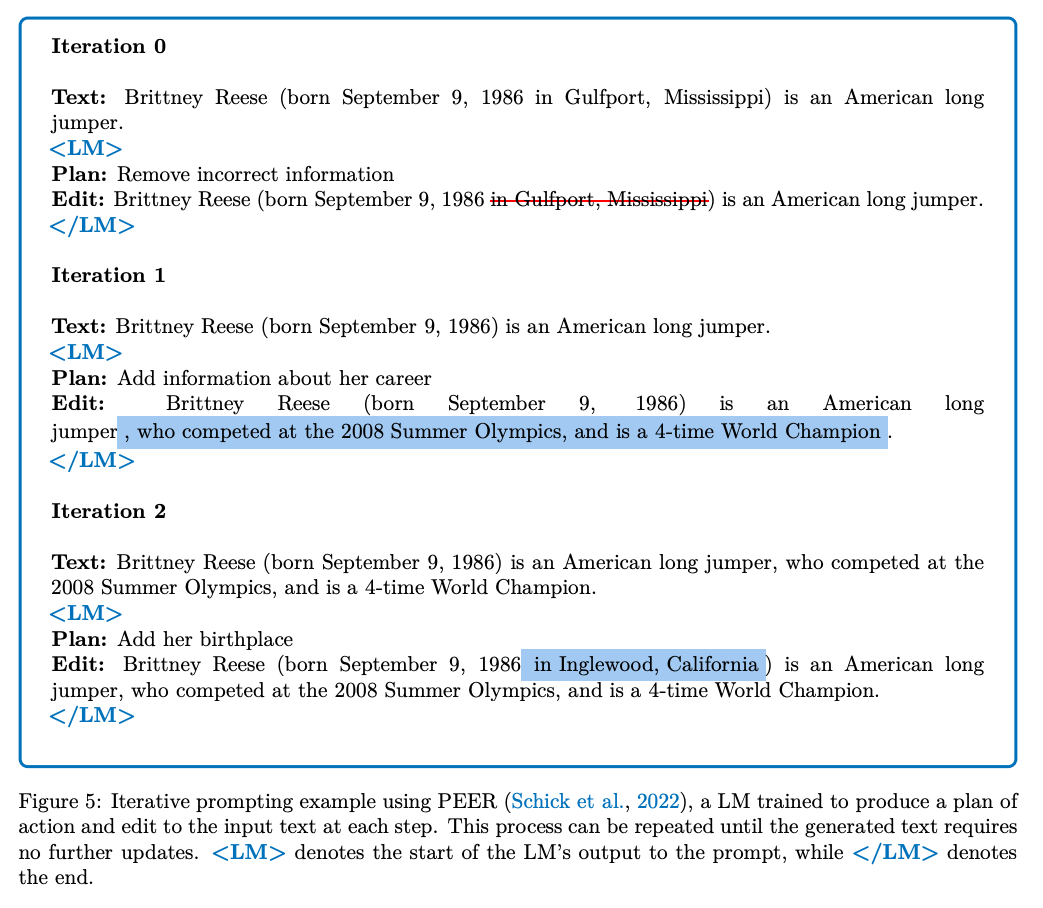
\includegraphics[width=\linewidth,keepaspectratio]{chatgpt46}
		\end{center}
    \end{column}
  \end{columns}
{\tiny (Ref: Overview of Large Language Models - Aman AI)}

\end{frame}

%%%%%%%%%%%%%%%%%%%%%%%%%%%%%%%%%%%%%%%%%%%%%%%%%%%%%%%%%%%
\begin{frame}[fragile]\frametitle{Retrieval/Knowledge-Augmented LLMs}

The first step is to convert internal documents into a query-friendly format by embedding them using an embedding model.

\begin{itemize}
\item LLMs can gain external knowledge through information retrieval from memory units like external databases.
\item There are two types of information retrievers: dense and sparse.
\item Sparse retrievers use a sparse bag-of-words representation for documents and queries.
\item Dense (neural) retrievers utilize dense query and document vectors obtained from a neural network.
\item Retrieval-augmented LMs have shown strong performance in knowledge-intensive tasks, closing the performance gap compared to larger LMs with more parameters.
\item Save the text representing each embedding along with its corresponding pointer for future reference.
\end{itemize}

{\tiny (Ref: Overview of Large Language Models - Aman AI)}

\end{frame}

%%%%%%%%%%%%%%%%%%%%%%%%%%%%%%%%%%%%%%%%%%%%%%%%%%%%%%%%%%%
\begin{frame}[fragile]\frametitle{Retrieval/Knowledge-Augmented LLMs}

Architecture of the system:


		\begin{center}
		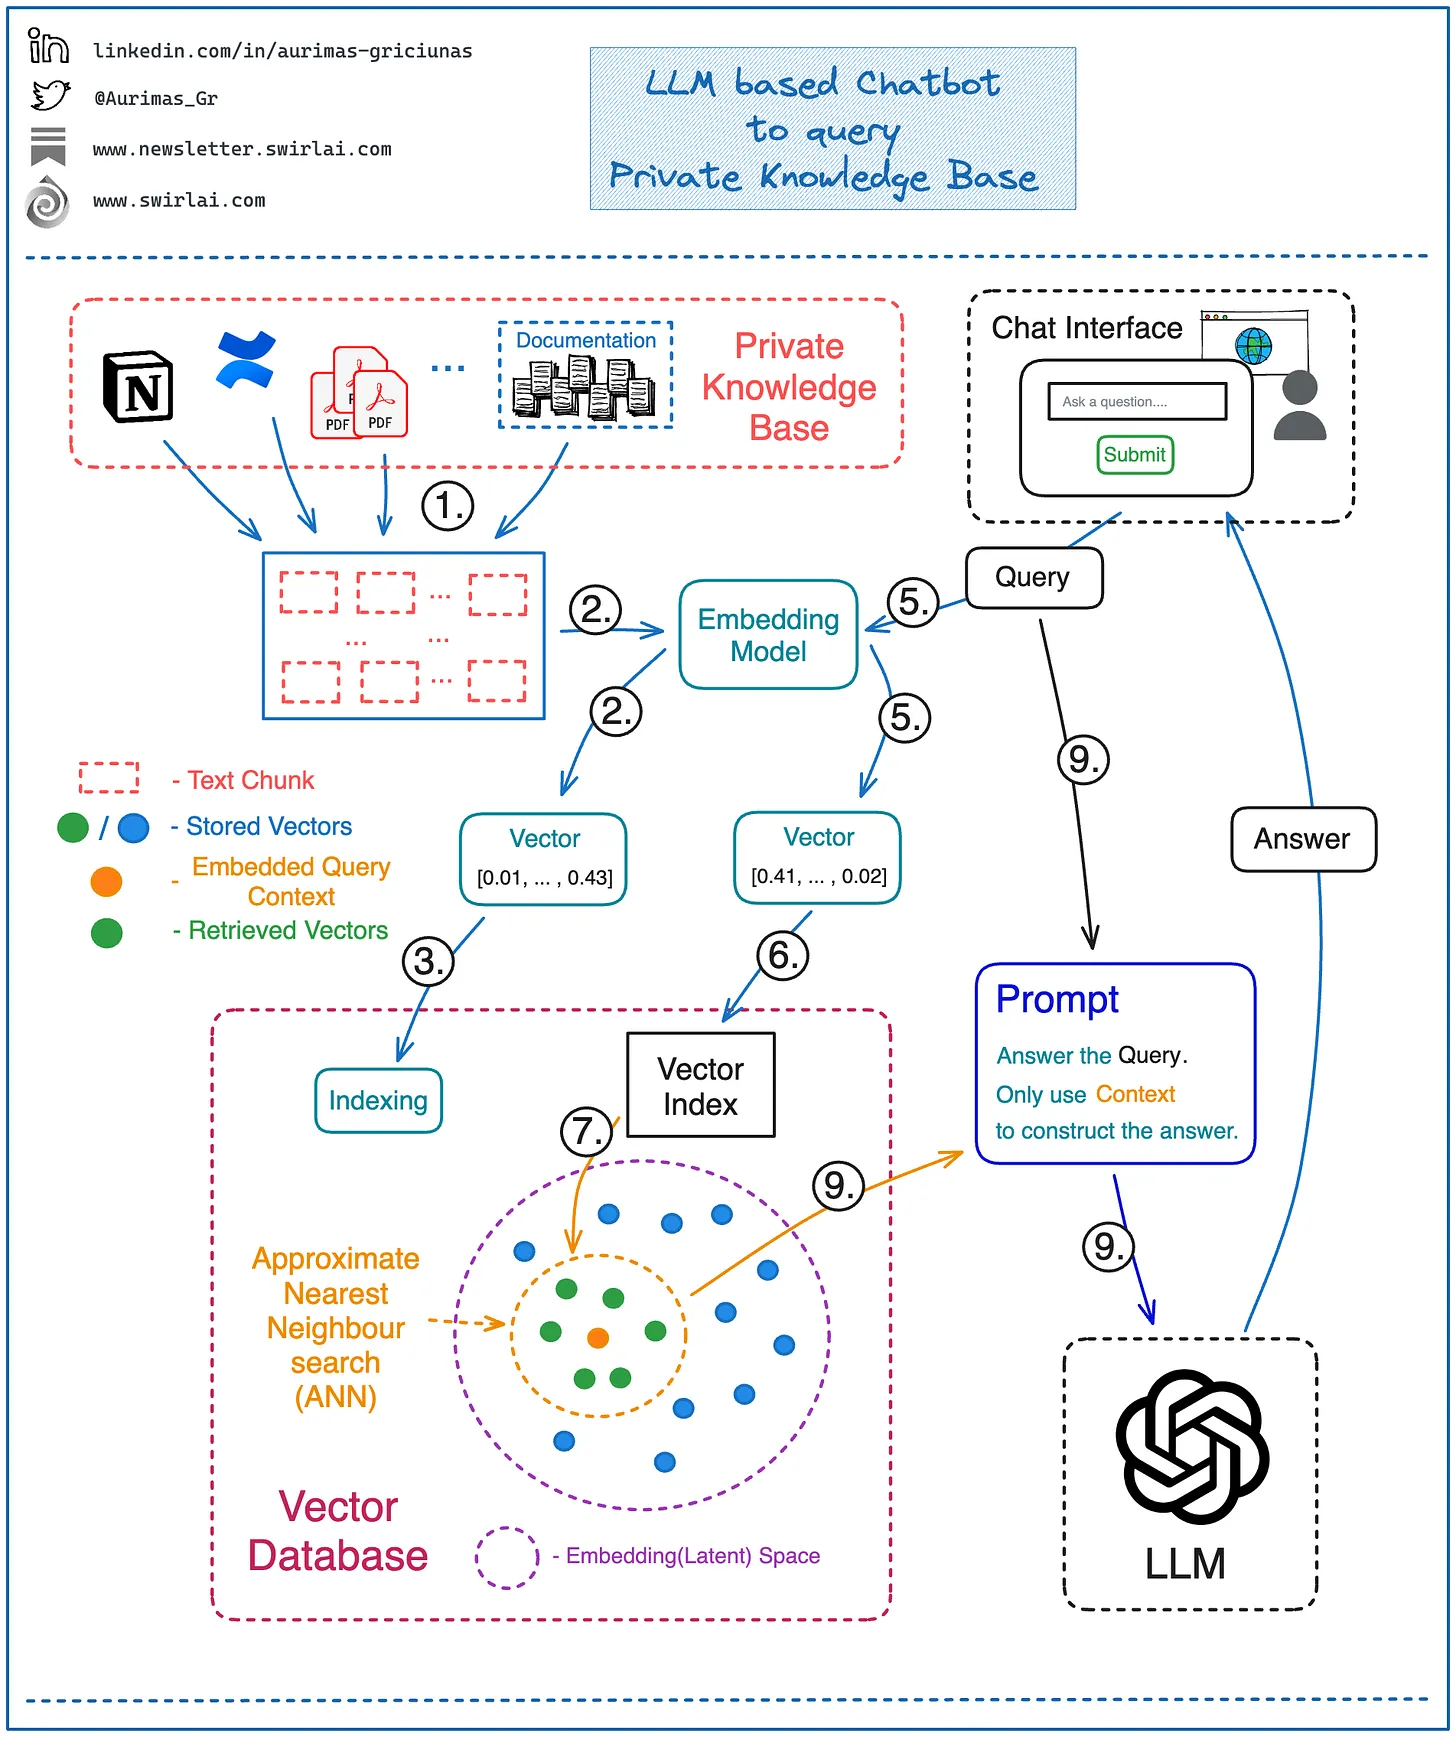
\includegraphics[width=\linewidth,keepaspectratio]{chatgpt47}
		\end{center}

{\tiny (Ref: Overview of Large Language Models - Aman AI)}

\end{frame}

%%%%%%%%%%%%%%%%%%%%%%%%%%%%%%%%%%%%%%%%%%%%%%%%%%%%%%%%%%%
\begin{frame}[fragile]\frametitle{Retrieval/Knowledge-Augmented LLMs}

The first step is to convert internal documents into a query-friendly format by embedding them using an embedding model.

\begin{itemize}
\item LLMs can gain external knowledge through information retrieval from memory units like external databases.
\item There are two types of information retrievers: dense and sparse.
\item Sparse retrievers use a sparse bag-of-words representation for documents and queries.
\item Dense (neural) retrievers utilize dense query and document vectors obtained from a neural network.
\item Retrieval-augmented LMs have shown strong performance in knowledge-intensive tasks, closing the performance gap compared to larger LMs with more parameters.
\item Save the text representing each embedding along with its corresponding pointer for future reference.
\end{itemize}

{\tiny (Ref: Overview of Large Language Models - Aman AI)}

\end{frame}

%%%%%%%%%%%%%%%%%%%%%%%%%%%%%%%%%%%%%%%%%%%%%%%%%%%%%%%%%%%
\begin{frame}[fragile]\frametitle{Retrieval/Knowledge-Augmented LLMs}

Next we can start constructing the answer to a question/query of interest:

\begin{itemize}
\item Embed the question using the same Embedding Model as the knowledge base.
\item Use the resulting Vector Embedding to query the Vector Database and specify the desired number of retrieved vectors, representing the context for answering the query.
\item Perform an Approximate Nearest Neighbour (ANN) search in the Vector DB to find similar vectors in the Embedding/Latent space.
\item Map the returned Vector Embeddings to the corresponding text chunks.
\item Provide the question and retrieved context text chunks to the LLM via prompt, instructing it to use only the provided context for answering the question.
\item Ensure that prompt engineering is applied to ensure the LLM's answers are within expected boundaries, avoiding fabricated answers when there is no relevant data in the retrieved context.
\end{itemize}

{\tiny (Ref: Overview of Large Language Models - Aman AI)}

\end{frame}

%%%%%%%%%%%%%%%%%%%%%%%%%%%%%%%%%%%%%%%%%%%%%%%%%%%%%%%%%%%
\begin{frame}[fragile]\frametitle{Retrieval/Knowledge-Augmented LLMs}

Next we can start constructing the answer to a question/query of interest:

\begin{itemize}
\item Use retrieval augmented generation (RAG) to enhance the knowledge base of an LM with relevant documents.
\item Employ vector databases like Pinecone, Chroma, Weaviate, Milvus, or LlamaIndex to augment LLMs.
\item RAG step-by-step process:
	\begin{itemize}
	\item Chunk, embed, and index documents in a vector database (VDB).
	\item Utilize (approximate) nearest neighbor techniques to match the query embedding of the claim advisor.
	\item Retrieve the relevant context from the VDB.
	\item Augment the LLM's prompt with the retrieved content.
	\end{itemize}

\item Consider LangChain or Google Vertex for prototyping or industrial applications, respectively.
\item Another approach is leveraging the search engine itself, as demonstrated by WebGPT, which can interact with a web browser, refine queries, navigate webpages, follow links, and cite sources.e within expected boundaries, avoiding fabricated answers when there is no relevant data in the retrieved context.
\end{itemize}

{\tiny (Ref: Overview of Large Language Models - Aman AI)}

\end{frame}

%%%%%%%%%%%%%%%%%%%%%%%%%%%%%%%%%%%%%%%%%%%%%%%%%%%%%%%%%%%
\begin{frame}[fragile]\frametitle{Retrieval/Knowledge-Augmented LLMs}

Next we can start constructing the answer to a question/query of interest:

\begin{itemize}
\item Interact with the LLM through an API or direct interaction when working with prompts.
\item Configure parameters to customize prompt results:

\begin{itemize}
\item Temperature: Lower temperature values increase determinism, selecting the highest probable next token. Higher values introduce more randomness, encouraging diversity and creativity in outputs. Lower temperature can be suitable for fact-based QA, while higher temperature may benefit creative tasks like poem generation.
\item Top\_p: Using nucleus sampling, top\_p controls the determinism of the model's response generation. Lower values prioritize exact and factual answers, while higher values promote diverse responses.
\end{itemize}

\item It is generally recommended to modify only one parameter at a time.
\item Results may vary depending on the specific version of the LLM used.
\end{itemize}

{\tiny (Ref: Overview of Large Language Models - Aman AI)}

\end{frame}

%%%%%%%%%%%%%%%%%%%%%%%%%%%%%%%%%%%%%%%%%%%%%%%%%%%%%%%%%%%
\begin{frame}[fragile]\frametitle{Methods to Knowledge-Augment LLMs}

Let’s look at a few methodologies to knowledge-augment LLMs

\begin{itemize}
\item Few-shot prompting: Powerful method for teaching LM desired outputs without weight updates; LM's reasoning and acting abilities tied to provided prompts.
\item Fine-tuning: Complementary to few-shot prompting; update weights of parameters via supervised learning.
\item Prompt pre-training: Mixing pre-training data with labeled demonstrations of reasoning to avoid overfitting during fine-tuning; empirical studies on gains compared to separate fine-tuning stage needed.
\item Bootstrapping: Prompting LM in few-shot setup, discarding examples where actions or reasoning steps didn't lead to correct final prediction.
\item Reinforcement Learning: Effective for teaching models to reason and act, utilizing supervised learning from human-created prompts.
\end{itemize}

{\tiny (Ref: Overview of Large Language Models - Aman AI)}

\end{frame}

%%%%%%%%%%%%%%%%%%%%%%%%%%%%%%%%%%%%%%%%%%%%%%%%%%%%%%%%%%%
\begin{frame}[fragile]\frametitle{Augmenting LLMs with Knowledge Graphs: Motivation}

\begin{itemize}
\item The Butcher-on-the-Bus: Rhetorical device highlighting human memory processes.
\item Memory Types: Two types of memory: flexible, fuzzy, and gradually learned vs. specific, precise, and acquired in a single shot.
\item Enhancing AI Systems: LLMs offer generalization and creativity but suffer from hallucinations, unreliability, and staleness. Databases provide accuracy and reliability but lack adaptability and intelligence.
\item Bridging the Gap: Integrating LLMs with Knowledge Graphs (KGs) to create a Working Memory Graph (WMG) combines the strengths of both approaches.
\item WMG Construction: LLM processes a question, returns a graph of nodes using URLs as identifiers, and links to ground truths in the KG. Conceptual understanding nodes connect LLM's vectors with KG's ontological classes.
\item Favorable Direction: Combining LLMs' reasoning capabilities with KGs' structured ontology can lead to promising exploration.
\end{itemize}

Thus, combining the best of both worlds (LLMs with their reasoning capabilities along with KGs with their structured, static ontology) can yield a favorable direction to explore.

{\tiny (Ref: Per Tony Seale, Overview of Large Language Models - Aman AI)}

\end{frame}

%%%%%%%%%%%%%%%%%%%%%%%%%%%%%%%%%%%%%%%%%%%%%%%%%%%%%%%%%%%
\begin{frame}[fragile]\frametitle{LangChain: Build Apps with LLMs}

\begin{itemize}
\item LangChain: Open-source framework for building applications with LLMs.
\item Capabilities: Enhances LLMs with prompt templates and integration of different APIs and external databases.
\item Application Examples: Building chatbots, Q\&A platforms, and real-time natural language understanding applications.
\item Data Discovery: Index text data into a vector database, partition into chunks, encode chunks into embeddings, and search for data using cosine similarity.
\item Prompt Engineering: Insert users' questions within prompt templates, provide context through examples, and create prompts with multiple (prompt, answer) pairs if needed.
\item Tools and Memory: LLM can utilize tools like Google Search, Python REPL, etc., and remember previous discussions through memory.
\item Challenges: Juggling questions, prompt templates, data search, tools, plan of action, and memory for constructing meaningful prompts.
\item LangChain Benefits: Powerful LLMops tool with an abstracted interface, API connection to public LLMs, integration with various tools and vector databases.
\item Visual Summary: Flowchart depicting the entire process.
\end{itemize}

{\tiny (Ref: Overview of Large Language Models - Aman AI)}

\end{frame}

%%%%%%%%%%%%%%%%%%%%%%%%%%%%%%%%%%%%%%%%%%%%%%%%%%%%%%%%%%%
\begin{frame}[fragile]\frametitle{LangChain: Build Apps with LLMs}

		\begin{center}
		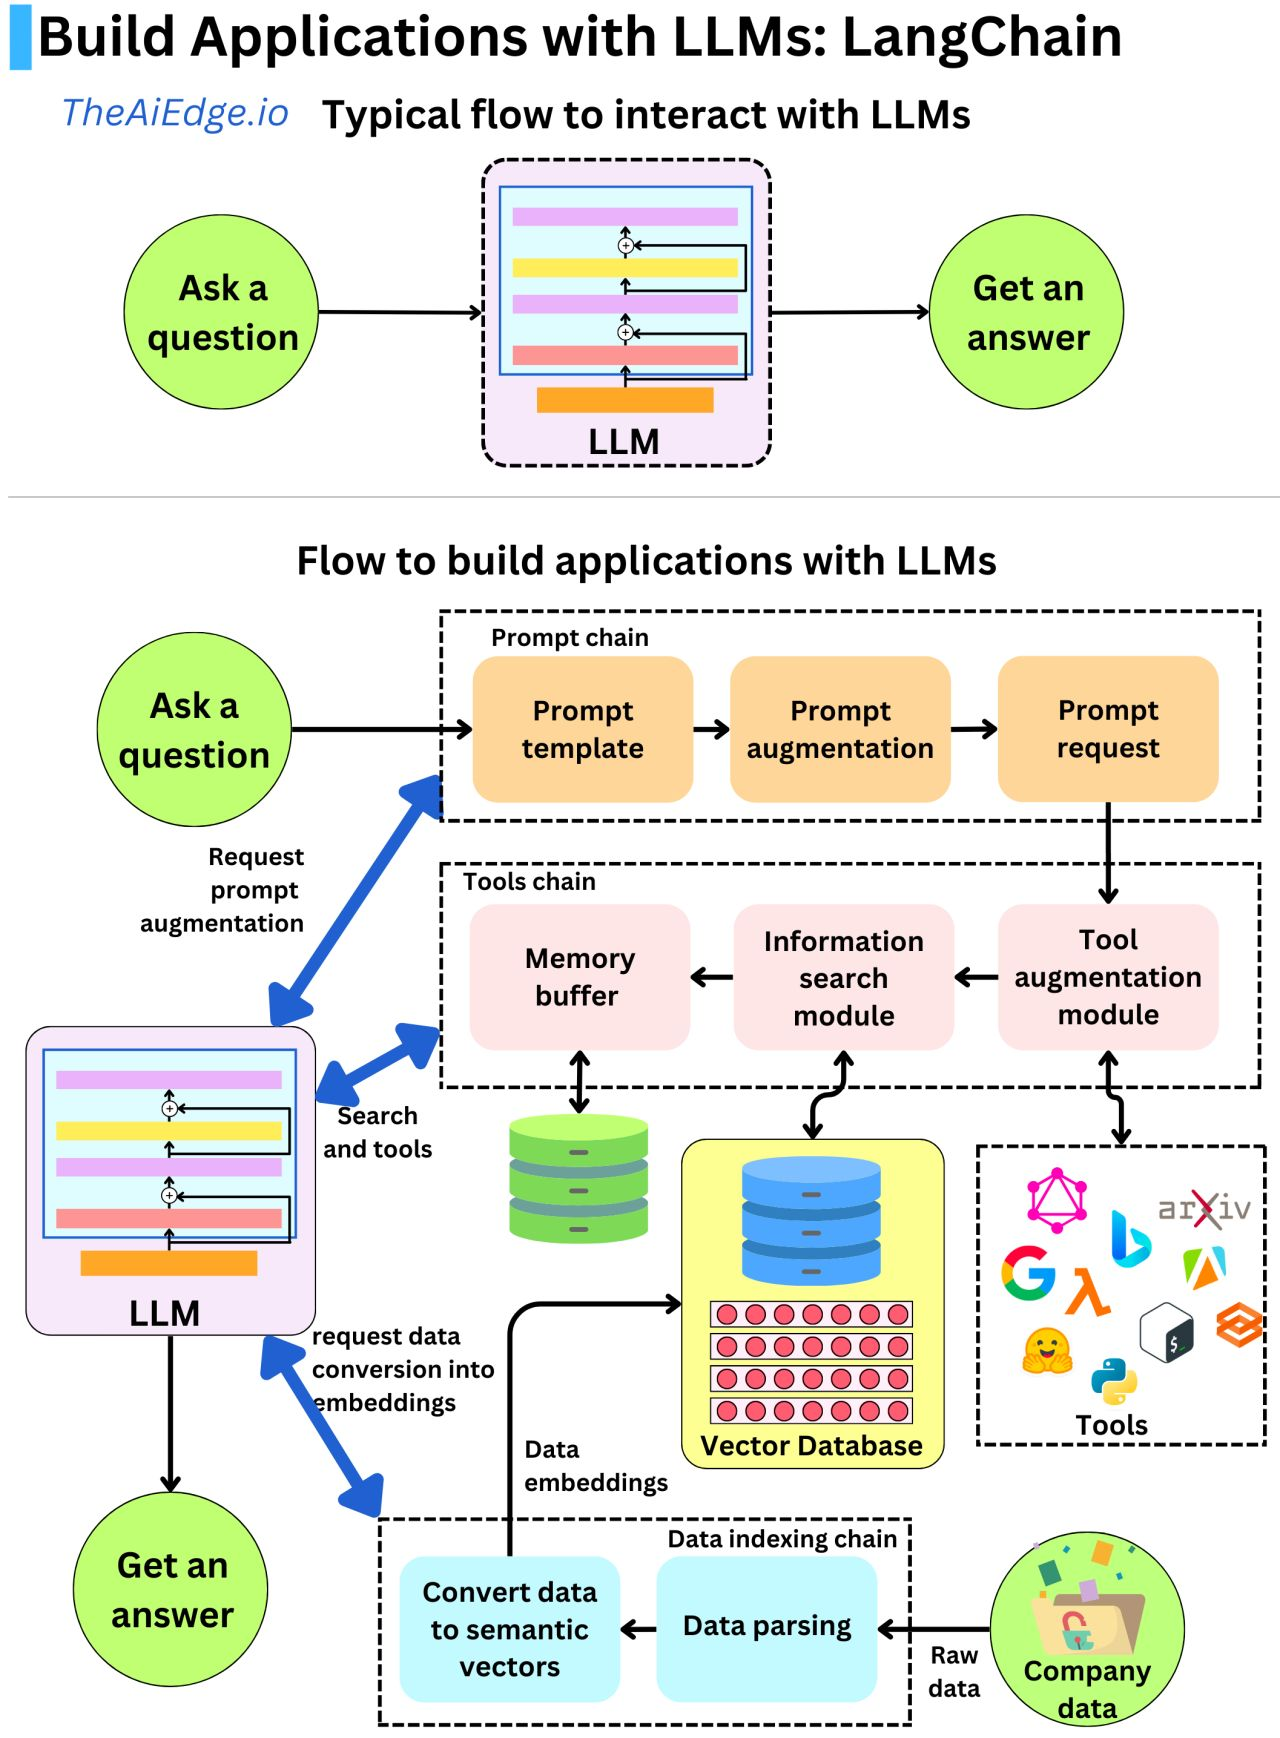
\includegraphics[width=\linewidth,keepaspectratio]{chatgpt48}
		\end{center}
		
{\tiny (Ref: Overview of Large Language Models - Aman AI)}

\end{frame}

%%%%%%%%%%%%%%%%%%%%%%%%%%%%%%%%%%%%%%%%%%%%%%%%%%%%%%%%%%%
\begin{frame}[fragile]\frametitle{Strategies to Get Better Results Using Prompt Engineering}

\begin{itemize}
\item Write clear instructions: Be specific about the desired length, format, or persona for the output. For example, you can ask the model to provide a 3-4 sentence summary in a formal tone, or adopt the persona of a witty comedian while generating a response.
\item Provide reference text: Include relevant reference text that can guide the model and improve the accuracy of the output. Reference materials can be used as study notes, helping the model stay on track and avoid hallucinated responses.
\item Break down complex tasks: Divide complex tasks into smaller subtasks to improve accuracy. For example, if handling an inbound support request, first use an API call to categorize the message, and then generate a response based on the category identified. Breaking down the task into manageable steps reduces error rates and yields better results.
\item Encourage thinking: Prompt the LLM to outline its thinking process to promote reasoning and improve response accuracy. By asking the model to explain its thought process, you can guide it towards more accurate and logical outputs.
\item Leverage external tools: Complement the capabilities of the LLM by utilizing external tools. For instance, integrate a text retrieval system or a code execution engine. You can even generate code with GPT to call external APIs for performing specific tasks. This combination of GPT and external tools expands the model's capabilities.
\item Evaluate changes systematically: Iteratively refine the prompt for optimal performance. Establish a comprehensive test suite that represents real-world usage, contains diverse test cases, and can be automated or repeated easily. Use this test suite to evaluate and compare the model's outputs against benchmark answers. Evaluations can involve computer-based assessments, human assessments, or a combination of both to ensure improvements in performance.
\end{itemize}

{\tiny (Ref: Overview of Large Language Models - Aman AI)}

\end{frame}